% !Mode:: "TeX:UTF-8"
\chapter{Lie Group and Lie Algebra}
\label{cpt:4}
\begin{mdframed}
    \textbf{Main Goal}
    \begin{enumerate}
        \item Understand the concept of Lie group, Lie algebra, and their applications of $ \mathrm{SO}( 3 ), \mathrm{SE}( 3 ) $ and the corresponding Lie algebras.
        \item Understands the meaning of BCH formula.
        \item Learn the perturbation model on Lie algebra.
        \item Use Sophus to perform operations on Lie algebras.
    \end{enumerate}
\end{mdframed}

In the last lecture, we introduced the description of rigid body motion in the three-dimensional world, including the rotation matrix, rotation vector, Euler angle, quaternion and so on. We focus on the representation of rotation, but in SLAM we have to estimate and optimize them in addition to the representation. Because the pose is unknown in SLAM, we need to solve the problem of ``\textbf {which camera pose best matches the current observation}''. A typical way is to build it into an optimization problem, solving the optimal $ \mathbf{R}, \mathbf{t}$ , and minimizing the error.

As mentioned before, the rotation matrix itself is constrained (orthogonal and the determinant is 1). When used as optimization variables, it introduces additional constraints on matrices that makes optimization difficult. Through the transformation relationship between Lie group and Lie algebra, we are able to turn the pose estimation into an unconstrained optimization problem and simplify the solution. Considering that the reader may not have the basic knowledge of Lie Group and Lie algebra, we will start with the most basic knowledge.

\newpage
\section{Basics of Lie Group and Lie Algebra}
In the last lecture, we introduced the definition of the rotation matrix and the transformation matrix. At the time, we said that the three-dimensional rotation matrix constitutes \textbf{special orthogonal group} $\mathrm{SO}(3)$, and the transformation matrix constitutes \textbf{special Euclidean group} $\mathrm{SE}(3) $. They are written like this:
\begin{equation}
\mathrm{SO}(3) = \{ \mathbf{R} \in \mathbb{R}^{3 \times 3} | \mathbf{RR}^\mathrm{T} = \mathbf{I}, \det(\mathbf{R})=1 \}.
\end{equation}
\begin{equation}
\mathrm{SE}(3) = \left\{ \mathbf{T} = \left[ {\begin{array}{*{20}{c}}
    \mathbf{R} & \mathbf{t} \\
    {{\mathbf{0}^\mathrm{T}}} & 1
    \end{array}} \right]
\in \mathbb{R}^{4 \times 4} | \mathbf{R} \in \mathrm{SO}(3), \mathbf{t} \in \mathbb{R}^3\right\}.
\end{equation}

However, at the time we did not explain the meaning of \textbf{group} in detail. Readers should note that both of the rotation matrix and the transformation matrix \textbf{are not closed to addition}. In other words, for any two rotation matrices $\mathbf{R}_1, \mathbf{R}_2$, according to the definition, their addition is no longer a rotation matrix:
\begin{equation}
\mathbf{R}_1 + \mathbf{R}_2 \notin \mathrm{SO}(3), \quad \mathbf{T}_1 + \mathbf{T}_2 \notin \mathrm{SE}(3).
\end{equation}
You can also say that the two matrices do not have a well-defined addition operator, or the matrix addition is not closed in these two sets. We find they have only one closed operation: the multiplication:
\begin{equation}
\mathbf{R}_1 \mathbf{R}_2 \in \mathrm{SO}(3), \quad \mathbf{T}_1 \mathbf{T}_2 \in \mathrm{SE}(3).
\end{equation}
We know that the matrix multiplication corresponds to the composition of two rotations or transformations. For a set that only has one ``well-defined'' operation, we call it a \textbf{group}.

\subsection{Group}
For the next contents we need to talk about a little bit abstract algebra. I think this is a necessary condition for discussing Lie Group and Lie Algebra, but in fact, except for the students of mathematics and physics, most of the students will not have this knowledge in undergraduate classes. So let's look at some basic concepts first.

A group is an algebraic structure of \textbf{a set} plus \textbf{an operation}. We denote the set as $A$ and the operation as $\cdot$, then the group can be denoted as $G=(A,\cdot)$. We say $G$ is a \textbf{group} if the operation satisfies the following conditions:

\begin{enumerate}
    \item { {Closure}}: $ \  \forall a_1, a_2 \in A, \  a_1 \cdot a_2 \in A$.
    \item { {Combination}}: $ \  \forall a_1, a_2, a_3 \in A, \  (a_1 \cdot a_2) \cdot a_3 = a_1 \cdot ( a_2 \cdot a_3) $.
    \item { {Unit element}}: $ \  \exists a_0 \in A, \  \mathrm{s.t.} \ \forall a \in A, \  a_0 \cdot a = a \cdot a_0 = a $.
    \item { {Inverse element}}: $ \  \forall a \in A, \  \exists a^{-1} \in A, \  st \  a \cdot a^{-1} = a_0 $.
\end{enumerate}

It is easy to verify that the rotation matrix set with the normal matrix multiplication form a group, and the same for transformation matrix with matrix multiplication, so they can be called as rotation matrix group and transformation matrix group. Other common groups include the addition of integers $(\mathbb{Z}, +)$, the rational numbers with multiplication after removing 0 $(\mathbb{Q}\backslash 0, \cdot )$, etc. Common groups in the matrix are:

\begin{itemize}
    \item {General Linear group $\mathrm{GL}(n)$}. The invertible matrix of $n \times n$ with matrix multiplication.
    \item {Special Orthogonal Group $\mathrm{SO}(n)$}. Or the rotation matrix group, where $\mathrm{SO}(2)$ and $\mathrm{SO}(3) $ is the most common.
    \item {Special Euclidean group $\mathrm{SE}(n)$}. Or the $n$ dimensional transformation described earlier, such as $\mathrm{SE}(2)$ and $\mathrm{SE}(3)$.
\end{itemize}

The group structure guarantees that the operations on the group have very good properties, and the \textbf{group theory} is the theory that studies the various structures and properties of the groups. Readers interested in group theory can refer to any of the modern algebra books. \textbf{Lie Group} refers to a group with continuous (smooth) properties. Discrete groups like the integer group $\mathbb{Z}$ have no continuous properties, so they are not Lie groups. And obviously, $\mathrm{SO}(n)$ and $\mathrm{SE}(n)$ are continuous in real space because we can intuitively imagine that a rigid body moving continuously in space, so they are all Lie Groups. Since $\mathrm{SO}(3)$ and $\mathrm{SE}(3)$ are especially important for camera pose estimation, we mainly discuss these two Lie groups. However, strictly discussing the concepts of ``continuous'' and ``smooth'' requires knowledge of analysis and topology, but we are not mathematics books, so only some important conclusions directly related to SLAM are introduced. If the reader is interested in the theoretical nature of Lie Groups, please refer to the special books like \cite{Varadarajan2013}.

Normally we have two ways to introduce the Lie Groups or Lie Algebras. The first is to directly introduce Lie group and Lie algebra, and then tell the reader that each Lie group corresponds to a Lie algebra, but in this case, the reader will think that Lie algebra seems to be a symbol that jumps out with no reason, and does not know its physical meaning. So, I am going to take a little time to draw the Lie algebra from the rotation matrix, similar to the practice of \cite{Ma2012}. Let's start with the simpler $\mathrm{SO}(3)$, leading to the Lie algebra $\mathfrak{so}(3)$ above $\mathrm{SO}(3)$.

\subsection{Introduction of the Lie Algebra}
Consider an arbitrary rotation matrix $\mathbf{R}$, we know that it satisfies:
\begin{equation}
\mathbf{R} \mathbf{R}^\mathrm{T}=\mathbf{I}.
\end{equation}
Now, we say that $\mathbf{R}$ is the rotation of a camera that changes continuously over time, which is a function of time: $\mathbf{R}(t)$. Since it is still a rotation matrix, we have
\[
\mathbf{R}(t) \mathbf{R}(t) ^T = \mathbf{I}.
\]
Deriving time on both sides of the equation yields (we use $\dot{\mathbf{R}}$ to represent the derivative of $\mathbf{R}$ on time $t$, just like many control books):
\[
\dot{\mathbf{R}} (t) \mathbf{R} {(t)^\mathrm{T}} + \mathbf{R} (t) \dot{\mathbf{R}} {(t) ^\mathrm{T}} = 0.
\]
Put the second item to right:
\begin{equation}
\dot{\mathbf{R}} (t) \mathbf{R} {(t)^\mathrm{T}} = - \left( \dot{\mathbf{R}} (t) \mathbf{R} {(t)^\mathrm{T}} \right)^\mathrm{T} .
\end{equation}

It can be seen that $\dot{\mathbf{R}} (t) \mathbf{R} {(t)^\mathrm{T}}$ is a \textbf{skew-symmetric} matrix. Recall that we introduced the $^\wedge$ symbol when we mention about the cross product in \eqref{eq:cross}, which turns a vector into an skew-symmetric matrix. Similarly, for any skew-symmetric matrix, we can also find a unique vector corresponding to it. Let this operation be represented by the symbol $^{\vee}$:
\begin{equation}
{\mathbf{a}^ \wedge } = \mathbf{A} = \left[ {\begin{array}{*{20}{c}}
    0&{ - {a_3}}&{{a_2}}\\
    {{a_3}}&0&{ - {a_1}}\\
    { - {a_2}}&{{a_1}}&0
    \end{array}} \right], \quad
{ \mathbf{A}^ \vee } = \mathbf{a}.
\end{equation}

So, since $\dot{\mathbf{R}} (t) \mathbf{R} {(t)^\mathrm{T}}$ is an skew-symmetric matrix, we can find a three-dimensional vector $\boldsymbol{\phi} (t) \in \mathbb{R}^3$ corresponds to it:
\[
\dot{\mathbf{R}} (t) \mathbf{R}(t)^\mathrm{T} = \boldsymbol{\phi} (t) ^ {\wedge}.
\]

Right multiply with $\mathbf{R}(t)$ on both sides, since $\mathbf{R}$ is an orthogonal matrix, we have:
\begin{equation}
\label{eq:dR}
\dot{\mathbf{R}} (t) = \boldsymbol{\phi} (t)^{\wedge} \mathbf{R}(t) =
\left[ {\begin{array}{*{20}{c}}
    0&{ - {\phi _3}}&{{\phi _2}}\\
    {{\phi _3}}&0&{ - {\phi _1}}\\
    { - {\phi _2}}&{{\phi _1}}&0
    \end{array}} \right] \mathbf{R} (t).
\end{equation}

It can be seen that we can take the time derivative of a ration matrix just by multiplying a $\boldsymbol{\phi}^\wedge (t)$ matrix on the left. Consider at time $t_0=0$, and the rotation matrix is $\mathbf{R}(0) = \mathbf{I}$. According to the derivative definition, $\mathbf{R}(t)$ can be used to perform a first-order Taylor expansion around $t=0$:
\begin{equation}
\begin{aligned}
\mathbf{R} \left( t \right) & \approx \mathbf{R} \left( t_0 \right) + \dot {\mathbf{R}} \left( {{t_0}} \right)\left ( {t - {t_0}} \right)\\
&= \mathbf{I} + \boldsymbol{\phi} {\left( {{t_0}} \right)^ \wedge } \left( t \right).
\end{aligned}
\end{equation}

We see that $\boldsymbol{\phi}$ reflects the derivative of $\mathbf{R}$, so it is called the \textbf{Tangent Space} near the origin of $\mathrm{SO}(3)$. Also, if time $t$ is close to $t_0$, we assume $\boldsymbol{\phi}(t)$ to close to be a constant $\boldsymbol{\phi}(t_0) = \boldsymbol{\phi}_0$. Then according to the formula \eqref{eq:dR}, we have:
\[
\dot{\mathbf{R}} (t) = \boldsymbol{\phi} (t_0) ^ {\wedge} \mathbf{R}(t) \approx \boldsymbol{\phi}_0^ {\wedge} \mathbf {R}(t).
\]

The above formula is a differential equation for $\mathbf{R}$, and with the initial value $\mathbf{R}(0) = \mathbf{I}$, we have solution like:
\begin{equation}
\label{eq:so3ode}
\mathbf{R}(t) = \exp \left( \boldsymbol{\phi}_0^\wedge t \right).
\end{equation}

The reader can verify that the above equation holds for both the differential equation and the initial value. This means that around $t = 0$, the rotation matrix can be calculated from $\exp \left( \boldsymbol{\phi}_0^\wedge t \right)$\footnote{At this point we have not explained what this $\exp$ means and how it works. We will talk about its definition and calculation process right after this section. }. We see that the rotation matrix $\mathbf{R}$ is associated with another skew-symmetric matrix $\boldsymbol{\phi}_0^\wedge t$ through an exponential relationship. But what is the exponential of a matrix? Here we have two questions that need to be clarified:

\begin{enumerate}
    \item Given $\mathbf{R}$ at a certain moment, we can find a $\boldsymbol{\phi}$ that describes the local derivative relationship of $\mathbf{R}$. How are they correlated with each other? We will say that $\boldsymbol{\phi}$ corresponds to the Lie algebra $\mathfrak{so}(3)$ on $\mathrm{SO}(3)$;
    \item Second, when a vector $\boldsymbol{\phi}$ is given, how is $\exp (\boldsymbol{\phi} ^\wedge )$ calculated? Conversely, given $\mathbf{R}$, is there an opposite operation to calculate $\boldsymbol{\phi}$? In fact, this is the exponential/logarithmic mapping between Lie group and Lie algebra.
\end{enumerate}

Let's solve these two problems below.

\subsection{The Definition of Lie Algebra}
Now let's give the strict definition of Lie Algebra. Each Lie group has a Lie algebra corresponding to it. Lie algebra describes the local structure of the Lie group around it origin point, or in other words, is the tangent space. The general definition of Lie algebra is listed as follows:

A Lie algebra consists of a set $\mathbb{V}$, a scalar field $\mathbb{F}$, and a binary operation $[,]$. If they satisfy the following properties, then $(\mathbb{V}, \mathbb{F}, [,])$ is a Lie algebra, denoted as $\mathfrak{g}$.

\begin{enumerate}
    \item Closure.  $\forall \mathbf{X}, \mathbf{Y} \in \mathbb{V}, [\mathbf{X}, \mathbf{Y}] \in \mathbb{V}$.
    \item Bilinear. $\forall \mathbf{X},\mathbf{Y},\mathbf{Z} \in \mathbb{V}, a,b \in \mathbb{F }, $ we have:
    \[
    [a\mathbf{X}+b\mathbf{Y}, \mathbf{Z}] = a[\mathbf{X}, \mathbf{Z}] + b [ \mathbf{Y}, \mathbf{Z} ], \quad [\mathbf{Z}, a \mathbf{X}+b\mathbf{Y}] = a [\mathbf{Z}, \mathbf{X} ]+ b [\mathbf{Z},\mathbf{Y}] .
    \]
    \item Reflexive \footnote{ Reflexive means that an element operates with itself results in zero. } $\forall \mathbf{X} \in \mathbb{V}, [\mathbf{X},\mathbf{X}] = \mathbf{0}$.
    \item Jacobi equation. $\forall \mathbf{X},\mathbf{Y},\mathbf{Z} \in \mathbb{V}, [\mathbf{X}, [ \mathbf{Y},\mathbf{Z}] ] + [\mathbf{Z}, [\mathbf{X},\mathbf{Y}] ] + [\mathbf{Y}, [\mathbf{Z}, \mathbf{X}]] =\mathbf{0}$.
\end{enumerate}
The binary operation $[,]$ is called \textbf{Lie brackets}. On the first glance, we require a lot of properties about the operator of Lie bracket.  Compared to the simpler binary operations in the group, the Lie bracket expresses the difference between the two elements. It does not require a combination law, but requires the element and itself to be zero after the brackets. As an example, the cross product $\times$ defined on the 3D vector $\mathbb{R}^3$ is a kind of Lie bracket, so $\mathfrak{g} = (\mathbb{R}^3, \mathbb{R}, \times)$ constitutes a Lie algebra. The reader can try to substitute the cross product into the above four properties to verify the above conclusion.

\subsection{Lie Algebra $\mathfrak{so}(3)$}
The previously mentioned $\boldsymbol{\phi}$ is actually a kind of Lie algebra. The Lie algebra corresponding to $\mathrm{SO}(3)$ is a vector defined on $\mathbb{R}^3$, which we will denote as $\boldsymbol{\phi}$. According to the previous derivation, each $\boldsymbol{\phi}$ can generate an skew-symmetric matrix:
\begin{equation}
\label{eq:phi}
\boldsymbol{\varPhi} = \boldsymbol{\phi}^{\wedge} = \left[ {\begin{array}{*{20}{c}}
    0&{ - {\phi _3}}&{{\phi _2}}\\
    {{\phi _3}}&0&{ - {\phi _1}}\\
    { - {\phi _2}}&{{\phi _1}}&0
    \end{array}} \right] \in \mathbb{R}^{3 \times 3}.
\end{equation}

Under this definition, the two vectors $\boldsymbol{\phi}_1, \boldsymbol{\phi}_2$'s Lie brackets are:
\begin{equation}
[\boldsymbol{\phi}_1, \boldsymbol{\phi}_2] = \left( \mathbf{ \varPhi }_1 \mathbf{ \varPhi }_2 - \mathbf{ \varPhi }_2 \mathbf{ \varPhi }_1 \right)^\vee.
\end{equation}

The reader can verify that the Lie brackets under this definition satisfy the above properties. Since the vector $\boldsymbol{\phi}$ is one-to-one with the skew-symmetric matrix, we say the elements of $\mathfrak{so}(3)$ are three-dimensional vectors or three-dimensional skew-symmetric matrices, without any ambiguity:
\begin{equation}
\mathfrak{so}(3) = \left\{ \boldsymbol{\phi} \in \mathbb{R}^3 \ \text{or}\  \boldsymbol{\varPhi} = \boldsymbol{\phi^\wedge} \in \mathbb{ R}^{3 \times 3} \right\}.
\end{equation}
Some books also use the symbol $\widehat{\boldsymbol{\phi}}$ to represent $\boldsymbol{\phi}^\wedge$, but the meaning is the same. At this point, we have made it clear about the contents of $\mathfrak{so}(3)$. They are just a set of \textbf{3D vectors} which can be used to express the derivative of the rotation matrix. Its relationship to $\mathrm{SO}(3)$ is given by the exponential map:
\begin{equation}
\mathbf{R} = \exp ( \boldsymbol{\phi}^\wedge ).
\end{equation}
The exponential map will be introduced later. Since we have introduced $\mathfrak{so}(3)$, we will first look at the corresponding Lie algebra on $\mathrm{SE}(3)$.

\subsection{Lie Algebra $\mathfrak{se}(3)$}
For $\mathrm{SE}(3)$, it also has a corresponding Lie algebra $\mathfrak{se}(3)$. To save space, I won't start by taking time derivatives. Similar to $\mathfrak{so}(3)$, $\mathfrak{se}(3)$ is located in the $\mathbb{R}^6$ space:
\begin{equation}
\mathfrak{se}(3) = \left\{ { \boldsymbol{\xi} = \left[ \begin{array}{l}
    \boldsymbol{\rho} \\
    \boldsymbol{\phi}
    \end{array} \right]
    \in { \mathbb{R}^6} ,
    \boldsymbol{\rho} \in { \mathbb{R}^3}, \boldsymbol{\phi} \in \mathfrak{so} \left( 3 \right),{ \boldsymbol{\xi} ^ \wedge } = \left[ {\begin{array}{*{20}{c}}
        {{ \boldsymbol{\phi} ^ \wedge }}& \boldsymbol{\rho} \\
        {{\mathbf{0}^\mathrm{T}}}&0
        \end{array}} \right] \in { \mathbb{R}^{4 \times 4}}} \right\}.
\end{equation}
We write each $\mathfrak{se}(3)$ element as $\boldsymbol{\xi}$, which is a six-dimensional vector. The first three dimensions are ``translation part'' (but keep in mind that the meaning is \textbf{different} from the translation in the transformation matrix, we will see later), which is denoted as $\boldsymbol{\rho}$; after the three-dimensional rotation, there is a $\boldsymbol{\phi}$, which is essentially a $\mathfrak{so}(3)$ element\footnote{Please note that in some books the authors may put the rotation in front and the translation in the back, which has no significant difference.}. At the same time, we extended the meaning of the $^\wedge$ symbol. In $\mathfrak{se}(3)$, a six-dimensional vector is also converted to a four-dimensional matrix using the $^\wedge$ symbol, but no longer a skew-symmetric one:
\begin{equation}
{ \boldsymbol{\xi} ^ \wedge } = \left[ {\begin{array}{*{20}{c}}
    {{ \boldsymbol{\phi} ^ \wedge }}& \boldsymbol{\rho} \\
    {{\mathbf{0}^\mathrm{T}}}&0
    \end{array}} \right] \in { \mathbb{R}^{4 \times 4}}.
\end{equation}

We still use the $^\wedge$ and $^\vee$ symbols to refer to the relationship from ``vector to matrix'' and ``matrix to vector'' to maintain consistency with $\mathfrak{so}(3)$. They are still one-to-one correspondence. The readers can simply take $\mathfrak{se}(3)$ as a ``vector consisting of a translation plus a $\mathfrak{so}(3)$ element'' (although $\boldsymbol{\rho} $ is not the direct translation). Similarly, the Lie algebra $\mathfrak{se}(3)$ also has a Lie bracket similar to $\mathfrak{so}(3)$:
\begin{equation}
[ \boldsymbol{\xi}_1, \boldsymbol{\xi}_2 ] = \left( \boldsymbol{\xi}_1^\wedge \boldsymbol{\xi}_2^\wedge -\boldsymbol{\xi}_2^ \wedge \boldsymbol{\xi}_1^\wedge \right) ^\vee.
\end{equation}

The reader can verify that it satisfies the definition of Lie algebra (I'll leave it as an exercise). So far we have seen two important Lie algebras $\mathfrak{so}(3)$ and $\mathfrak{se}(3)$.

\section{Exponential and Logarithmic Mapping}
\subsection{Exponential Map of $\mathrm{SO}(3)$}

Now consider the second question: How to calculate $\exp ( \boldsymbol{\phi}^{\wedge} )$? Obviously it is an exponential map of a matrix. Again, we will first discuss the exponential mapping of $\mathfrak{so}(3)$ and then the case of $\mathfrak{se}(3)$.

The exponential of an arbitrary matrix can be written as a Taylor expansion if it is converged, whose result is still a matrix:
\begin{equation}
\exp(\mathbf{A}) = \sum\limits_{n = 0}^\infty {\frac{1}{{n!}}{ \mathbf{A}^n}}.
\end{equation}

Similarly, for any element in $\boldsymbol{\phi} \in \mathfrak{so}(3)$,, we can also define its exponential map in this way:
\begin{equation}
\exp(\boldsymbol{\phi}^\wedge) = \sum\limits_{n = 0}^\infty {\frac{1}{{n!}}{ (\boldsymbol{\phi}^{\wedge })^n}}.
\end{equation}
But this definition cannot be calculated directly because we don't want to calculate the infinite power of a matrix. Below we derive a convenient way to calculate the exponential mapping. Since $\boldsymbol{\phi}$ is a three-dimensional vector, we can define its length and direction,  denoted as $\theta$ and $\mathbf{a}$, respectively. So we have $\boldsymbol{\phi} = \theta \mathbf{a}$, where $\mathbf{a}$ is a unit-length direction vector, i.e., $\| \mathbf{a} \| =1$. First, for such a unit-length vector $\mathbf{a}$, there are two properties: 
\begin{equation}
 \mathbf{a}^{\wedge} \mathbf{a}^{\wedge} = \left[ {\begin{array}{*{20}{c}}
{ - a_2^2 - a_3^2}&{{a_1}{a_2}}&{{a_1}{a_3}}\\
{{a_1}{a_2}}&{ - a_1^2 - a_3^2}&{{a_2}{a_3}}\\
{{a_1}{a_3}}&{{a_2}{a_3}}&{ - a_1^2 - a_2^2}
\end{array}} \right] = \mathbf{a} \mathbf{a}^\mathrm{T} - \mathbf{I},
\end{equation}
as well as
\begin{equation}
\mathbf{a}^{\wedge} \mathbf{a}^{\wedge} \mathbf{a}^{\wedge} = \mathbf{a}^\wedge (\mathbf{a}\mathbf{a} ^\mathrm{T}-\mathbf{I}) = - \mathbf{a}^{\wedge}.
\end{equation}
These two formulas provide a way to handle the high-order $\mathbf{a}^\wedge$ items. Now we can write the exponential map as:
\begin{align*}
\exp \left( {{\boldsymbol{\phi} ^ \wedge }} \right) &= \exp \left( {\theta {\mathbf{a}^ \wedge }} \right) = \sum\limits_ {n = 0}^\infty {\frac{1}{{n!}}{{\left( {\theta {\mathbf{a}^ \wedge }} \right)}^n}} \\
&= \mathbf{I} + \theta {\mathbf{a}^ \wedge } + \frac{1}{{2!}}{\theta ^2}{\mathbf{a}^ \wedge }{\ Bm{a}^ \wedge } + \frac{1}{{3!}}{\theta ^3}{\mathbf{a}^ \wedge }{\mathbf{a}^ \wedge }{\mathbf{ a}^ \wedge } + \frac{1}{{4!}}{\theta ^4}{\left( {{\mathbf{a}^ \wedge }} \right)^4} + ... \\
&= \mathbf{a} {\mathbf{a}^\mathrm{T}} - {\mathbf{a}^ \wedge }{\mathbf{a}^ \wedge } + \theta {\mathbf{a} ^ \wedge } + \frac{1}{{2!}}\theta^2 {\mathbf{a}^ \wedge }{\mathbf{a}^ \wedge } - \frac{1}{{3! }}{\theta ^3}{\mathbf{a}^ \wedge } - \frac{1}{{4!}}{\theta ^4}{\left( {{\mathbf{a}^ \wedge }} \right)^2} + ...\\
&= \mathbf{a}{\mathbf{a}^\mathrm{T}} + \underbrace{\left( {\theta - \frac{1}{{3!}}{\theta ^3} + \ Frac{1}{{5!}}{\theta ^5} - ...} \right)}_{\sin \theta} {\mathbf{a}^ \wedge } - \underbrace{\left( { 1 - \frac{1}{{2!}}{\theta ^2} + \frac{1}{{4!}}{\theta ^4} - ...} \right)}_{\cos \theta}{\mathbf{a}^ \wedge }{\mathbf{a}^ \wedge }\\
&= {\mathbf{a}^ \wedge }{\mathbf{a}^ \wedge } + \mathbf{I} + \sin \theta {\mathbf{a}^ \wedge } - \cos \theta {\ Bm{a}^ \wedge }{\mathbf{a}^ \wedge }\\
&= (1 - \cos \theta ){\mathbf{a}^ \wedge }{\mathbf{a}^ \wedge } + \mathbf{I} + \sin \theta {\mathbf{a}^ \wedge }\\
&= \cos \theta \mathbf{I} + (1 - \cos \theta )\mathbf{a}{\mathbf{a}^\mathrm{T}} + \sin \theta {\mathbf{a}^ \wedge }.
\end{align*}

Finally, we got a very familiar equation:
\begin{equation}
\exp( \theta \mathbf{a}^\wedge ) = \cos \theta \mathbf{I} + (1 - \cos \theta )\mathbf{a}{\mathbf{a}^\mathrm{T} } + \sin \theta {\mathbf{a}^ \wedge }.
\end{equation}

Recall the previous lesson, this equation is exactly the same as the Rodriguez formula, i.e. equation \eqref{eq:rogridues}. This shows that $\mathfrak{so}(3)$ is actually the \textbf{rotation vector}, and the exponential map is the just the Rodriguez formula. Through them, we map any vector in $\mathfrak{so}(3)$ to a rotation matrix in $\mathrm{SO}(3)$. Conversely, if we define a logarithmic map, we can also map the elements in $\mathrm{SO}(3)$ to $\mathfrak{so}(3)$:
\begin{equation}
\boldsymbol{\phi} = \ln {\left( \mathbf{R} \right)^ \vee } = {\left( {\sum\limits_{n = 0}^\infty {\frac{{{{ \left( { - 1} \right)}^n}}}{{n + 1}}{{\left( { \mathbf{R} - \mathbf{I}} \right)}^{n + 1 }}} } \right)^ \vee }.
\end{equation}
Just like the exponential mapping, we don't have to use Taylor to expand the logarithmic mapping. In Lecture 3, we have already introduced how to calculate the corresponding Lie algebra according to the rotation matrix, that is, using the formula \eqref{eq:R2theta}, and use the properties of the trace to solve the rotation angle and the rotation axis separately, which is more convenient.

Now, we've introduced the calculation method of exponential mapping. Readers may ask, what is the property of the exponential mapping? Can I find a unique $\boldsymbol{\phi}$ for any $\mathbf{R}$? Unfortunately, the exponential map is just a surjective map, not injective. This means that for each element in $\mathrm{SO}(3)$ we can find a $\mathfrak{so}(3)$ element corresponding to it; however, there may be multiple $\mathfrak{so}(3)$ elements corresponding to the same $\mathrm{SO}(3)$ element. At least for the rotation angle $\theta$, we know that rotating multiple $360^\circ$ will give the same rotation - it has periodicity. However, if we fix the rotation angle between $\pm \pi$, then the Lie group and the Lie algebra elements are one-to-one correspondence.

The conclusion of $\mathrm{SO}(3)$ and $\mathfrak{so}(3)$ seems to be in our expectation. It is very similar to the rotation vector we talked about earlier, and the exponential mapping is the Rodrigues formula. The derivative of the rotation matrix can be specified by the rotation vector, which guides how to perform calculus operations in the rotation matrix.

\subsection{Exponential Map of $\mathrm{SE}(3)$}

The exponential map on $\mathfrak{se}(3)$ is described below. In order to save space, we no longer deduct the exponential mapping in detail like $\mathfrak{so}(3)$. The exponential mapping on $\mathfrak{se}(3)$ is as follows:
\begin{align}
\exp \left( {{ \boldsymbol{\xi} ^ \wedge }} \right) &= \left[ {\begin{array}{*{20}{c}}
    {\sum\limits_{n = 0}^\infty {\frac{1}{{n!}}{{\left( {{\boldsymbol{\phi} ^ \wedge }} \right)}^n} } }&{\sum\limits_{n = 0}^\infty {\frac{1}{{\left( {n + 1} \right)!}}{{\left( {{\boldsymbol{\phi } ^ \wedge }} \right)}^n} \boldsymbol{\rho} } }\\
    {{\mathbf{0}^\mathrm{T}}}&1
    \end{array}} \right] \\
&\buildrel \Delta \over = \left[ {\begin{array}{*{20}{c}}
    \mathbf{R} &{\mathbf{J\rho} } \\
    {{\mathbf{0}^\mathrm{T}}}&1
    \end{array}} \right] = \mathbf{T}.
\end{align}

With a little patience, you can derive the Taylor expansion from the practice of $\mathfrak{so}(3)$. Let $\boldsymbol{\phi}=\theta \mathbf{a}$, where $\mathbf{a}$ is the unit vector, then:
\begin{equation}
\begin{aligned}
\sum\limits_{n = 0}^\infty {\frac{1}{{\left( {n + 1} \right)!}}{{\left( {{\boldsymbol{\phi} ^ \wedge }} \right)}^n}} &= \mathbf{I} + \frac{1}{{2!}}\theta {\mathbf{a}^ \wedge } + \frac{1}{{3 !}}{\theta ^2}{\left( {{\mathbf{a}^ \wedge }} \right)^2} + \frac{1}{{4!}}{\theta ^3}{ \left( {{\mathbf{a}^ \wedge }} \right)^3} + \frac{1}{{5!}}{\theta ^4}{\left( {{\mathbf{a} ^ \wedge }} \right)^4} \cdots \\
&= \frac{1}{\theta }\left( {\frac{1}{{2!}}{\theta ^2} - \frac{1}{{4!}}{\theta ^4} + \cdots } \right)\left( {{\mathbf{a}^ \wedge }} \right) + \frac{1}{\theta }\left( {\frac{1}{{3!}} {\theta ^3} - \frac{1}{5}{\theta ^5} + \cdots } \right){\left( {{\mathbf{a}^ \wedge }} \right)^2} + \mathbf{I}\\
&= \frac{1}{\theta }\left( {1 - \cos \theta } \right)\left( {{\mathbf{a}^ \wedge }} \right) + \frac{{\theta - \sin \theta }}{\theta }\left( {\mathbf{a}{\mathbf{a}^T} - \mathbf{I}} \right) + \mathbf{I}\\
&= \frac{{\sin \theta }}{\theta }\mathbf{I} + \left( {1 - \frac{{\sin \theta }}{\theta }} \right)\mathbf{a }{\mathbf{a}^T} + \frac{{1 - \cos \theta }}{\theta }{\mathbf{a}^ \wedge } \buildrel \Delta \over = \mathbf{J}.
\end{aligned}
\end{equation}

From the results, we can see the $\mathbf{R}$ in the upper left corner of the exponential map of $\boldsymbol{\xi}$ is just the well-known $\mathrm{SO}(3)$, which means the rotation part of $\boldsymbol{\xi}$ is just the rotation part in $\mathfrak{so}(3)$. The $\mathbf{J}$ in the upper right corner is given by the above derivation:
\begin{equation}
\label{eq:lieAlgebraJacobian}
\mathbf{J} = \frac{{\sin \theta }}{\theta } \mathbf{I} + \left( {1 - \frac{{\sin \theta }}{\theta }} \right) \mathbf{a} { \mathbf{a}^\mathrm{T}} + \frac{{1 - \cos \theta }}{\theta }{ \mathbf{a}^ \wedge }.
\end{equation}

This formula is somewhat similar to the Rodrigues formula, but not exactly the same. We see that after passing the exponential map, the translation part is multiplied by a linear jacobian matrix $\mathbf{J}$. Please pay attention to the $\mathbf{J}$ here, as it will be used later.

Similarly, although we can also derive the logarithmic mapping analytically, there is a more trouble-free way to find the corresponding vector on $\mathfrak{so}(3)$ according to the transformation matrix $\mathbf{T}$: from the upper left corner $\mathbf{R}$ we can calculate the rotation vector, while $\mathbf{t}$ the upper right corner satisfies:
\begin{equation}
\mathbf{t} = \mathbf{J} \boldsymbol{\rho}.
\end{equation}

Since $\mathbf{J}$ can be obtained from $\boldsymbol{\phi}$, $\boldsymbol{\rho}$ can also be solved by this linear equation. Now, we have clarified the definition of Lie Group and Lie algebra and their mutual conversion relationship, as summarized in \autoref{fig:liegroupandAlgebra}~. If the reader doesn't understand everything, please go back to a few pages to look the formula derivation again.

\begin{figure}[!ht]
    \centering
    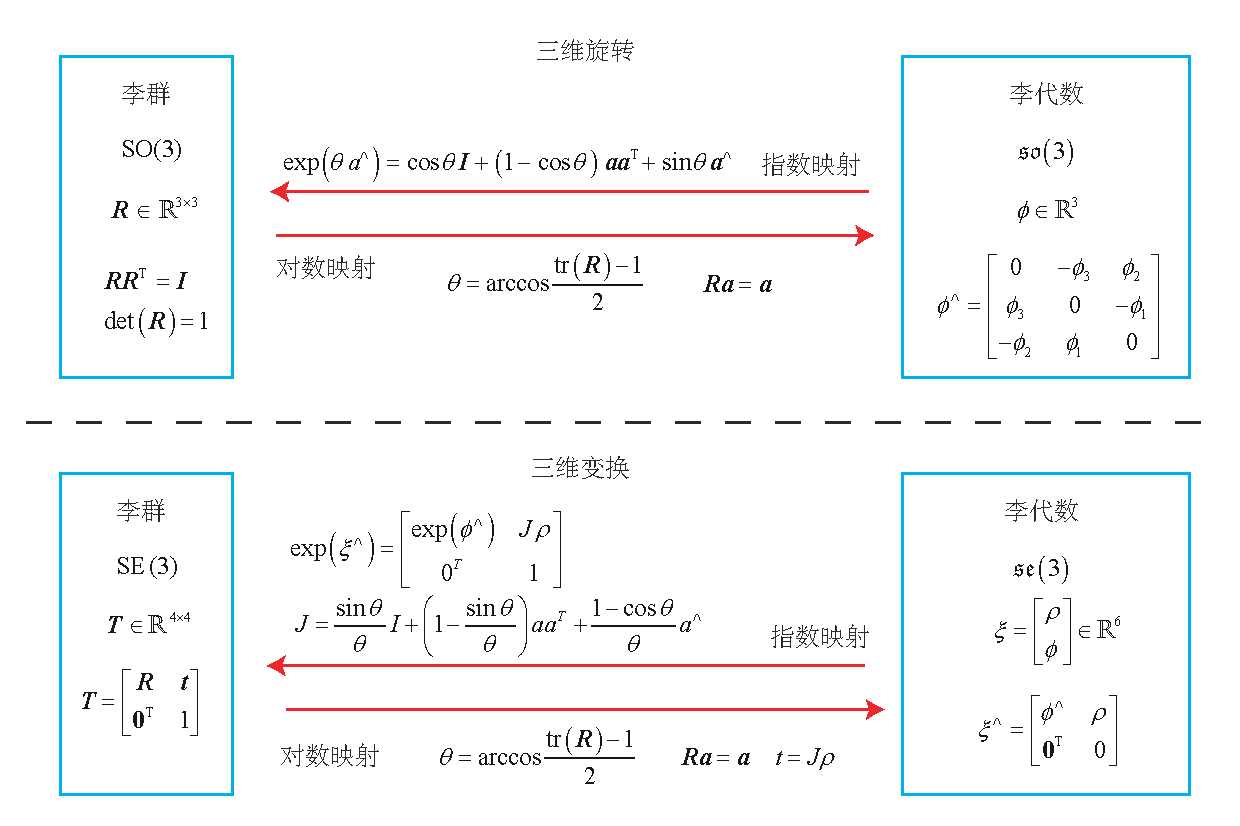
\includegraphics[width=1.0\textwidth]{lieGroup/liegroupandAlgebra.pdf}
    \caption{The correspondence between $\mathrm{SO}(3), \mathrm{SE}(3), \mathfrak{so}(3), \mathfrak{se}(3)$. }
    \label{fig:liegroupandAlgebra}
\end{figure}

\section{Lie Algebra Derivation and Perturbation Model}
\subsection{BCH Formula and its Approximation}
A major motivation for using Lie algebra is to do optimization, and the derivative is a very necessary information in the optimization process (we will talk about it in detail in Lecture 6). Let's consider a problem below. Although we have already understood the relationship between Lie group and Lie algebra on $\mathrm{SO}(3)$ and $\mathrm{SE}(3)$, but what happens in $\mathfrak{so}(3)$ when two matrix are multiplied in $\mathrm{SO}(3)$? Conversely, when we add two vectors in $\mathfrak{so}(3)$, does $\mathrm{SO}(3)$ correspond to the product of the two matrices? If we write it out, it should be:
\[
\exp \left( {\boldsymbol{\phi}_1^\wedge } \right)\exp \left( {\boldsymbol{\phi}_2^\wedge}\right) = \exp \left( {{{\left( {{\boldsymbol{\phi} _1} + {\boldsymbol{\phi} _2}} \right)}^ \wedge }} \right) ?
\]

If $\boldsymbol{\phi}_1, \boldsymbol{\phi}_2$ are scalars, then obviously this is true; but here we calculate the exponential function of \textbf{matrix} instead of a scalar. In other words, we are studying whether the following formula holds:
\[
\ln \left( \exp \left( \mathbf{A} \right) \exp \left( \mathbf{B} \right) \right) = \mathbf{A} + \mathbf{B} \; ?
\]
for matrices. Unfortunately, this formula is not true in the matrix. The complete form of the product is given by the Baker-Campbell-Hausdorff formula (BCH formula)\footnote{ See \url{https://en.wikipedia.org/wiki/Baker-Campbell-Hausdorff\_formula}. }. Due to the complexity of its complete form, we only give the first few items of its expansion:
\begin{equation}
\ln \left( {\exp \left( \mathbf{A} \right)\exp \left( \mathbf{B} \right)} \right) = \mathbf{A} + \mathbf{B} + \frac{1}{2}\left[ {\mathbf{A}, \mathbf{B}} \right] + \frac{1}{{12}}\left[ {\mathbf{A},\left[ {\mathbf{A}, \mathbf{B}} \right]} \right] - \frac{1}{{12}}\left[ {\mathbf{B},\left[ {\mathbf{A} ,\mathbf{B}} \right]} \right] + \cdots
\end{equation}
Where $[]$ is the Lie brackets. The BCH formula tells us that how to deal with the product of two matrices: they produce some extra Lie brackets compared with the scalar form. In particular, consider the case of $\mathrm{SO}(3)$, the $\ln { \left( {\exp \left( { \boldsymbol{\phi} _1^ \wedge } \right)\exp \left ( {\boldsymbol{\phi} _2^ \wedge } \right)} \right) ^ \vee }$, when $\boldsymbol{\phi_1}$ or $\boldsymbol{\phi_2}$ is small, small items with more than quadratic can be simply ignored. At this time, BCH has a linear approximation\footnote{We are not going to do the detailed derivation of BCH approximation, see \cite{Barfoot2016} if you are interested. }:
\begin{equation}
\ln { \left( {\exp \left( { \boldsymbol{\phi} _1^ \wedge } \right)\exp \left( {\boldsymbol{\phi} _2^ \wedge } \right)} \right ) ^ \vee } \approx \left\{
\begin{array}{l}
{\mathbf{J}_l}{\left( {{\boldsymbol{\phi} _2}} \right)^{ - 1}}{ \boldsymbol{\phi} _1} + {\boldsymbol{\phi} _2 } \quad \text{when} \ \boldsymbol{\phi}_1 \ \text{is a small amount},\\
{\mathbf{J}_r}{\left( {{\boldsymbol{\phi} _1}} \right)^{ - 1}}{\boldsymbol{\phi} _2} + {\boldsymbol{\phi} _1 } \quad \text{when} \  \boldsymbol{\phi}_2 \ \text{is a small amount}.
\end{array} \right.
\end{equation}

Take the first approximation as an example. This formula tells us to left multiply a tiny rotation matrix $\mathbf{R}_1$ on a rotation matrix $\mathbf{R}_2$ (whose Lie algebra is $\boldsymbol{\phi}_1$ and $\boldsymbol{\phi}_2$, respectively), in $\mathfrak{so}(3)$ it can be approximated by adding a $\mathbf{J}_l \left( {\boldsymbol{\phi} _2} \right)^{ - 1} { \boldsymbol{\phi} _1}$ to the original Lie algebra $\boldsymbol{\phi}_2$.  Similarly, the second approximation describes the case where $\mathbf{R}_1$ is right multiplied by a small rotation. Therefore, under the BCH approximation, the Lie algebra is divided into a left-multiplying approximation and a right-multiplying approximation. In daily usage, we must pay attention to whether the left model or the right model is used. This book takes the left multiplication as an example. The jacobian in our left model $\mathbf{J}_l$ is actually the content of the form \eqref{eq:lieAlgebraJacobian}~:
\begin{equation}
{ \mathbf{J}_l} = \mathbf{J} = \frac{{\sin \theta }}{\theta } \mathbf{I} + \left( {1 - \frac{{\sin \theta } }{\theta }} \right) \mathbf{a} { \mathbf{a}^\mathrm{T}} + \frac{{1 - \cos \theta }}{\theta }{ \mathbf{a} ^ \wedge}.
\end{equation}

Its inverse is:
\begin{equation}
\mathbf{J}_l^{ - 1} = \frac{\theta }{2}\cot \frac{\theta }{2} \mathbf{I} + \left( {1 - \frac{\theta } {2}\cot \frac{\theta }{2}} \right) \mathbf{a} {\mathbf{a}^\mathrm{T}} - \frac{\theta }{2}{ \mathbf{ a}^ \wedge }.
\end{equation}
if $\theta$ is not zero (in that case we take both $\mathbf{J}_{l}$ and its inverse as identity). To get the right jacobian we only need to take a negative sign for the argument:
\begin{equation}
\mathbf{J}_r(\boldsymbol{\phi}) =\mathbf{J}_l(-\boldsymbol{\phi}) .
\end{equation}

By this way, we've made it clear about the relationship between Lie group multiplication and Lie algebra addition.

For the convenience of the reader, we restate the meaning of the BCH approximation. Suppose we have a rotation $\mathbf{R}$, the corresponding Lie algebra is $\boldsymbol{\phi}$. We give it a small perturbation to the left, denoted as $\Delta \mathbf{R}$, and so that the corresponding Lie algebra is $\Delta \boldsymbol{\phi}$. Then, on Lie group, the result is $ \Delta \mathbf{R} \cdot \mathbf{R}$, and on the Lie algebra, according to the BCH approximation, it is $\mathbf{J}_l^{-1 } (\boldsymbol{\phi}) \Delta \boldsymbol{\phi} + \boldsymbol{\phi}$. Put them together, we can simply write:
\begin{equation}
\exp \left( {\Delta { \boldsymbol{\phi} ^ \wedge }} \right)\exp \left( {{ \boldsymbol{\phi} ^ \wedge }} \right) = \exp \left( {{{\left( { \boldsymbol{\phi} + \mathbf{J}_l^{ - 1}\left( \boldsymbol{\phi} \right)\Delta \boldsymbol{\phi} } \right)} ^ \wedge }} \right).
\end{equation}

Conversely, if we do addition on Lie algebra by adding $\boldsymbol{\phi}$ with $\Delta \boldsymbol{\phi}$, we can approximate the multiplication on the Lie group as:
\begin{equation}
\exp \left( {{{\left( { \boldsymbol{\phi} + \Delta \boldsymbol{\phi} } \right)}^ \wedge }} \right) = \exp \left( {{{\left( {{ \mathbf{J}_l}\Delta \boldsymbol{\phi} } \right)}^ \wedge }} \right)\exp \left( {{ \boldsymbol{\phi} ^ \wedge }} \right) = \exp \left( {{\boldsymbol{\phi} ^ \wedge }} \right)\exp \left( {{{\left( {{\mathbf{J}_r}\Delta \boldsymbol{ \phi} } \right)}^ \wedge }} \right).
\end{equation}

This provides a theoretical basis for calculus on Lie algebra. Similarly, for $\mathrm{SE}(3)$, there is a similar BCH approximation:
\begin{equation}
\exp \left( {\Delta {\boldsymbol{\xi} ^ \wedge }} \right)\exp \left( {{ \boldsymbol{\xi} ^ \wedge }} \right) \approx \exp \left ( {{{\left( {{ \boldsymbol{\mathcal{J}}_l^{-1} }\Delta \boldsymbol{\xi} + \boldsymbol{\xi} } \right)}^ \wedge }} \right),
\end{equation}
\begin{equation}
\exp \left( {{ \boldsymbol{\xi} ^ \wedge }} \right) \exp \left( {\Delta {\boldsymbol{\xi} ^ \wedge }} \right) \approx \exp \left ( {{{\left( {{ \boldsymbol{\mathcal{J}}_r^{-1} }\Delta \boldsymbol{\xi} + \boldsymbol{\xi} } \right)}^ \wedge }} \right).
\end{equation}

Here the $\boldsymbol{\mathcal{J}}_l$ is a more complicated $6 \times 6$ matrix. Readers can find its detailed contents in \cite{Barfoot2016}. Since we did not use the jacobians in the calculation (we will see in the next subsection), the exact form is omitted here.